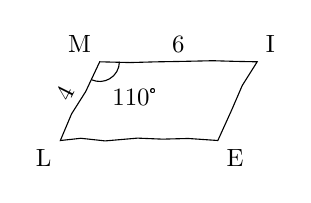
\begin{tikzpicture}[rotate=0,every node/.style={scale=0.9},scale=0.5]

\coordinate (M) at (0,0);
\coordinate (I) at (4,0);
\coordinate (E) at (3,-2);
\coordinate (L) at (-1,-2);

\draw[decorate,decoration={random steps,amplitude=1pt,segment length=10pt}] (M) node [above left]{M}--(I) node [above right]{I}--(E) node [below right] {E}--(L) node [below left] {L}--cycle;

\draw (0.5,0) arc (0:-114:0.5);
\node at (0.9,-0.9){110°};

\path (M)--(L) node[midway,above,sloped]{4};
\path (M)--(I) node[midway,above]{6};
\end{tikzpicture}